\section{Chapter 17: The Beginning of Time}
\subsection{The Big Bang}
We can use light from distant galaxies to see about a billion years into the past, beyond this we cannot see any objects bright enough. We also run into a problem with background radiation left over from the Big Bang. This radiation is from when the universe was 380 000 years old (before that light could not pass through). Most of our knowledge of the Big Bang is from mathematical models.

\subsubsection{Conditions of the Early Universe}
During the first few seconds the universe was so hot that photons could transform themselves into matter and back. When two photons collide with energy twice that of a electron (its mass times $c^2$) they make a electron (matter) and positron (antimatter). When these two meet they annihilate each other and release photon energy. Similar actions can be done for protons and neutrons. At its start, the universe was full of matter and antimatter jumping to and from energy.

Forces:
\begin{itemize}
\item Gravity: holds planets together (dominant on large objects)
\item Electromagnetism: holds particles together (dominant on atoms and molecules)
\item Strong nuclear: holds atom nucleus together
\item Weak nuclear: deals with fusion and fission
\end{itemize}

At high temperatures (like at the birth of the universe) some of these meld into a different force. At its very start the universe was governed by one super force.

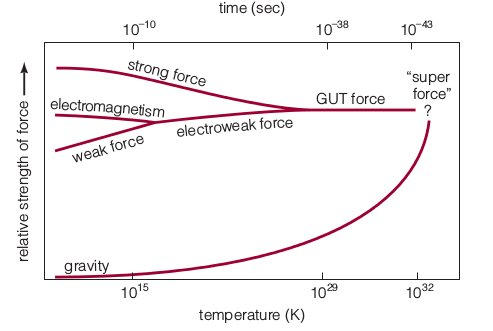
\includegraphics[scale=0.5]{forces}

\subsubsection{History of the Universe}
We break the history of the universe into eras.

\begin{wrapfigure}{l}{5.5cm}
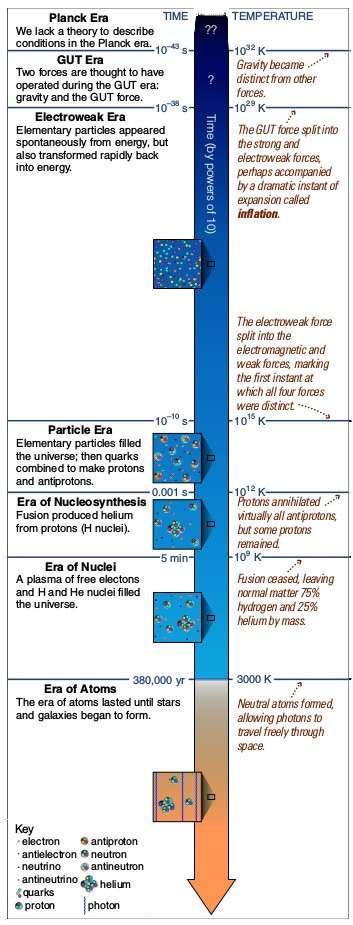
\includegraphics[width=5.5cm]{eras}
\end{wrapfigure}

\textbf{Planck Era}
This is the limit of what our current understanding of physics can explain. At this point we know that mass and energy were being converted back and forth rapidly. These energy fluctuations caused a changing gravitational field that warped space and time. A problem arises in that we have no theory to link quantum mechanics and general relativity. This era ended when the universe cooled enough for the super force to break into GUT force and gravity.

\textbf{GUT Era}
We know barely more about this era than we do about the Planck era, and even then what we know is not well tested. We think that the separation of GUT into strong and electroweak forces released a ton of energy causing a dramatic expansion of the universe called \textbf{inflation} (we think expanding things of atomic size to solar system sized).

\textbf{Electroweak Era}
At the end of this era the electroweak force breaks apart into the electromagentic and weak nuclear forces. This is the first point where we have experimental evidence of things actually fitting our models. Particle accelerators produced weak bosons that we predicted would exist during this era.

\textbf{Particle Era}
This is the era right before the crazy energy-particle switching calmed down. All of the quarks created during this era had combined into protons and neutrons by its end. Since we were not spontaneously making matter and antimatter the two started permanently annihilating each other. We know that matter out numbered antimatter because matter exists. By comparing estimates on how many protons and photons there are we can get a rough estimate of the size of matter antimatter imbalance. The two numbers would have been similar at the start of the universe, but now photons outnumber protons a billion to one. This means that for every billion antiprotons there were a billion and one protons so when the billion annihilated themselves they made a billion extra photons.

\textbf{Era of Nucleosynthesis}
Now that we had a steady amount of matter it started fusing into heavier elements but the heat of the universe kept breaking them apart. At the end of this era it had gotten too cool to fuse heavier elements.

\textbf{Era of Nucleus}
At this point the universe consisted of plasma made of hydrogen and helium nuclei and electrons. Light didnt really go anywhere because it just bounced around between electrons (like it does inside a star). At the end of this era the universe had cooled enough for the nuclei to snag electrons and become stable. Once that happened light could travel in straight lines.

\textbf{Era of Atoms and Era of Galaxies}
Now that we have stable atoms we can be in the era of atoms. The universe is now a mix of neutral atoms, plasma, and photons. Slight areas of higher density started attracting atoms and plasma to make protogalactic clouds. These went on to form stars and eventually galaxies. This is the era we are currently in.

\subsection{Evidence}
The big bang theory is widely accepted because it accurately predicts \textbf{cosmic background microwave radiation} as the radiation that started streaming through the universe at the end of the nuclei era. It also accurately predicts the amount of helium in the universe.

\subsubsection{Left Over Radiation}
Arno Penzias and Robert Wilson kept hearing noise on their microwave antenna, this was background radiation from the universes formation. They found that the noise was exactly the same from every direction (so it wasn't just coming from something). At the same time a group at Princton had found that the radiation created during the formation of the universe (predicted by George Gamow) would have to still exist and be detectable with microwave antennas.

Scientists predicted that cosmic background radiation would have a prefect thermal spectrum since it was from the start of the universe. Since it broke free when the universe was the temperature of a red giant it should have the same signature, but stretched by 1000 (since thats how much the universe has expanded since then). This shifted spectrum represents the temperature just above absolute 0. The Cosmic Background Explorer (COBE) satellite was launched to test these theories and it confirmed that cosmic background radiation has a perfect thermal spectrum and is about 3K. COBE also showed that background radiation is not absolutely the same in every direction. This had been a strike against the Big Bang Theory since the universe couldn't have been that smooth (it had to have pockets of slightly higher gravity for starts to form).

\subsubsection{Abundance of Elements}
Background radiation also explains a discrepancy in the amount of helium in a galaxy. No galaxy is $<25\%$ helium, but star fusion can only produce 10\% helium. This means that some helium must have been present during the formation of the universe, so the universe must have been hot enough at some point to fuse hydrogen. The temperature of the background radiation can be used to calculate how hot the universe was in the past and this can be used to calculate how much helium was fused (roughly 25\%).

During the formation of the universe it was hot enough to switch between protons and neutrons, but as it cooled the universe favored creating protons since neutrons are heavier. During this time protons and neutrons combined to form deuterium (weird hydrogen nucleus containing a neutron). Deuterium fused to form helium. Most of these were blown apart by gamma radiation but as the universe continued to cool some stuck around. Here protons outnumbered neutrons seven to one. All neutrons were incorporated into helium-4 atoms resulting in one helium (weight 4) for every 12 hydrogen (weight 1 each), so 25\% of the universe's weight was helium.

Rarely reactions could form lithium, but all other elements were created in stars. This is because by the time the universe has stable helium and hydrogen atoms to fuse into heavier elements it was too cool to fuse them.

\subsection{Inflation}
Lots of what we know about the origin of the universe is uncertain because we have no way to experimentally verify them.

\subsubsection{Mysteries}
Stuff we cannot explain with the Big Bang Theory without inflation:
\begin{itemize}
\item the structure: matter collected around areas of slightly higher density, where did these come from and why were they there
\begin{itemize}
\item we can experimentally prove that the energy fields at any point in space fluctuate slightly, these might cause density enhancements
\item inflation would have increased the wavelengths of these fluctuations to be large enough to generate the density enhancements that existed (based on background radiation calculations)
\end{itemize}
\item the uniformness: for something of its scale the universe is surprisingly smooth (varying by only 0.01\%)
\begin{itemize}
\item before inflation radiation was continuously bouncing around and interacting which lead to a normalization of it
\item inflation then flung this radiation far apart from each other very quickly so that they didn't have time to fuck with each other resulting in the smoothness we see
\end{itemize}
\item density id close to critical density: if we sum dark matter and dark energy we find that the universe density is far too close to the critical density to be a coincidence
\begin{itemize}
\item the universe is surprisingly flat which is only possible if its density was uniformly equal to the critical density (point at which kinetic expansion matched gravitational pull)
\item inflation explains this by expanding the universe so quickly that any curvature would not be noticeable on the scale of our universe
\end{itemize}
\end{itemize}
Note: inflation does not violate the speed of light since things aren't moving through a distance quickly, the distance itself is stretching.

\subsubsection{Testing Inflation}
We test inflation by using it to make predictions and seeing if its right (and it is);
\begin{itemize}
\item The overall geometry is flat, implying that the total mass-energy of the universe is equivalent to the critical density.
\item The density of ordinary matter is 4.6\% of the critical density, in agreement with observations of deuterium in the universe.
\item The total matter density is 28\% of the critical density. Subtracting the 4.6\% for ordinary matter, we conclude that dark matter, probably in the form of weakly interacting massive particles, makes up about 23\% of the critical density, in agreement with what we infer from measurements of the masses of clusters of galaxies.
\item The combination of a flat geometry and a matter density lower than the critical density implies the existence of a repulsive force due to dark energy that currently accelerates the expansion, in agreement with observations of distant supernovae. Because the total mass-energy of the universe is the critical density, and matter accounts for only 28\% of this, dark energy must account for the remaining 72\% of the mass-energy of the universe.
\item The universe’s age should be about 13.7 billion years at the current microwave temperature of 2.73 K, in agreement with what we infer from Hubble’s constant and the ages of the oldest stars.
\end{itemize}

\subsection{Observing the Big Bang}
They sky is dark at night. Duh. But this actually makes no sense. \textbf{Olber's Paradox} is that if the universe is infinite and unchanging, then the sky should be as bright as the sun. Since the universe is infinite in every direction, there should be almost no part of the sky that doesn't have a source of light in the way. Even with the explanation of dust and black holes, the sky is too dark. The Big Bang Theory explains this by saying we can only see a finite number of stars because the universe began at a particular moment so our field of vision is limited.
